%\documentstyle[epsf,twocolumn]{jarticle}       %LaTeX2.09仕様
%\documentclass[twocolumn]{jarticle}     %pLaTeX2e仕様
\documentclass[twocolumn]{jarticle}     %pLaTeX2e仕様

%一枚組だったら[twocolumn]関係のとこ消す

\setlength{\topmargin}{-45pt}
%\setlength{\oddsidemargin}{0cm} 
\setlength{\oddsidemargin}{-7.5mm}
%\setlength{\evensidemargin}{0cm} 
\setlength{\textheight}{24.1cm}
%setlength{\textheight}{25cm} 
\setlength{\textwidth}{17.4cm}
%\setlength{\textwidth}{172mm} 
\setlength{\columnsep}{11mm}

\kanjiskip=.07zw plus.5pt minus.5pt

\usepackage{graphicx}
\usepackage[dvipdfmx]{color}
\usepackage{subcaption}
\usepackage{enumerate}
\usepackage{comment}
\usepackage{url}
\usepackage{multirow}
\usepackage{diagbox}


\begin{document}
\twocolumn[
  \noindent
  \hspace{1em}

  \today
  \hfill
  \ \  B3 西村昭賢 

  \vspace{2mm}
  \hrule
  \begin{center}
  {\Large \bf 情報工学実験2 10/25 課題}
  \end{center}
  \hrule
  \vspace{3mm}
]

\section{実験内容}
scikit-learnライブラリを用いて,様々な分類モデルを作成し,性能評価を行った.

\subsection*{データセット}
用いたデータセットはscikit-learnライブラリに組み込まれているIrisデータセットを用いた.
「花びらの長さ」,「花びらの幅」の2つの特徴量を用いて,Iris-setosa,Iris-versicolor,Iris-virginicaの3つのラベルをを0,1,2と整数で符号化したクラスラベルに対して分類を行った.
\par
全体の30\%をテストデータ,その他70\%を学習データとしてデータセットをランダムに分割し実験を行った.
データを分割する際,クラスラベルの比率は入力データセットと等しくなるようにした.

\subsection*{用いたアルゴリズム}
分類モデルを作成する際,以下のアルゴリズムを用いた.

\begin{quote}
  \begin{itemize}
   \item パーセプトロン
   \item ロジスティック回帰
   \item 線形SVM
   \item カーネルSVM
   \item 決定木
   \item ランダムフォレスト
  \end{itemize}
 \end{quote}



\subsection*{性能評価}

モデルの性能を評価する際,テストデータセットを用いて,以下の指標で評価した.

\begin{quote}
  \begin{itemize}
    \item 混同行列(Confusion matrix)
   \item 正解率(Accuracy)
   \item 適合率(Precision)
   \item 再現率(Recall)
   \item F1値(F1-measure)
  \end{itemize}
 \end{quote}
 適合率,再現率,F1値に関しては各クラスごとと,分類結果全体の計算を行った.
なお分類結果全体の計算は,Irisデータセットにおいてラベルごとのデータの偏りは起こっていないためマクロ平均で行った.\cite{macro}

\section{実験結果}
各アルゴリズムを用いたモデルに対し,前節で述べた性能評価を行った結果を示す.
\subsection*{パーセプトロン}

図\ref{fig:パーセプトロン}にパーセプトロンにおける混同行列を示す.

\begin{figure}[ht]
  \centering
  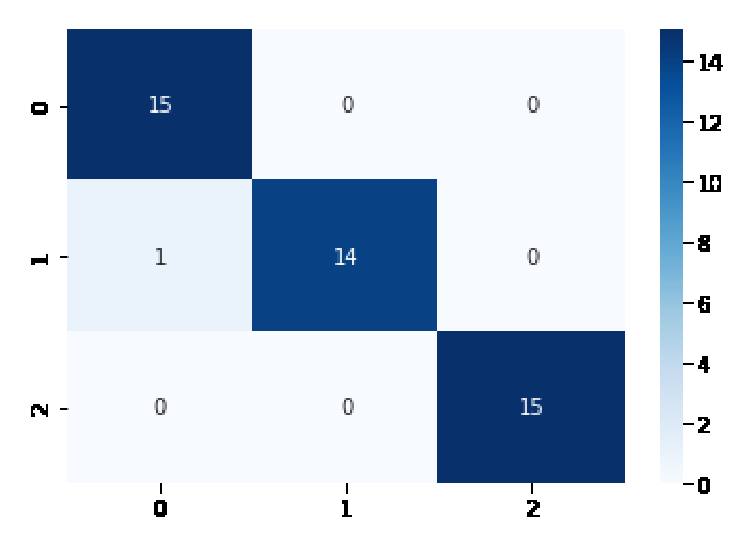
\includegraphics[width=80mm]{assets/ppn_heatmap.eps}
  \caption{パーセプトロン分類モデルにおける混同行列}
  \label{fig:パーセプトロン}
\end{figure}

正解クラスが0であるデータに対してクラス1と誤分類したデータが1つあることがわかる.\par
また,表\ref{table:パーセプトロン}にパーセプトロンモデルにおける正解率,適合率,再現率,F1値を示す.

\begin{table}[hbtp]
  \caption{パーセプトロンモデルにおける正解率,適合率,再現率,F1値}
  \label{table:パーセプトロン}
  \centering
  \begin{tabular}{lccc}
    \hline
     & Precision  &  Recall &  F1-measure \\
    \hline
    クラス0  & 0.93750  & 1.00000 & 0.96774 \\
    クラス1  & 1.00000  & 0.93333 & 0.96552 \\
    クラス2  & 1.00000  & 1.00000 & 1.00000 \\
    分類結果全体  &  0.97917  &  0.97778 & 0.97775 \\
    \hline
    Accuracy & & & 0.97778\\
    \hline
  \end{tabular}
\end{table}

\subsection*{ロジスティック回帰}

\subsection*{線形SNM}

\subsection*{カーネルSVM}

\subsection*{決定木}

\subsection*{ランダムフォレスト}







%index.bibはtexファイルと同階層に置く
%ちゃんと\citeしないと表示されない(1敗)
\bibliography{index.bib}
\bibliographystyle{junsrt}

\end{document}
